\documentclass[11pt]{article}
\usepackage[margin=1in]{geometry}
\usepackage{graphicx}
\usepackage{amsmath}
\usepackage{caption}

\title{HW1 A3: Polynomial Regression and the Effect of Regularization}
\author{CSEP 546}
\date{}

\begin{document}
\maketitle

\section*{Fitted Polynomial: Before and After Regularization}

\begin{figure}[h]
    \centering
    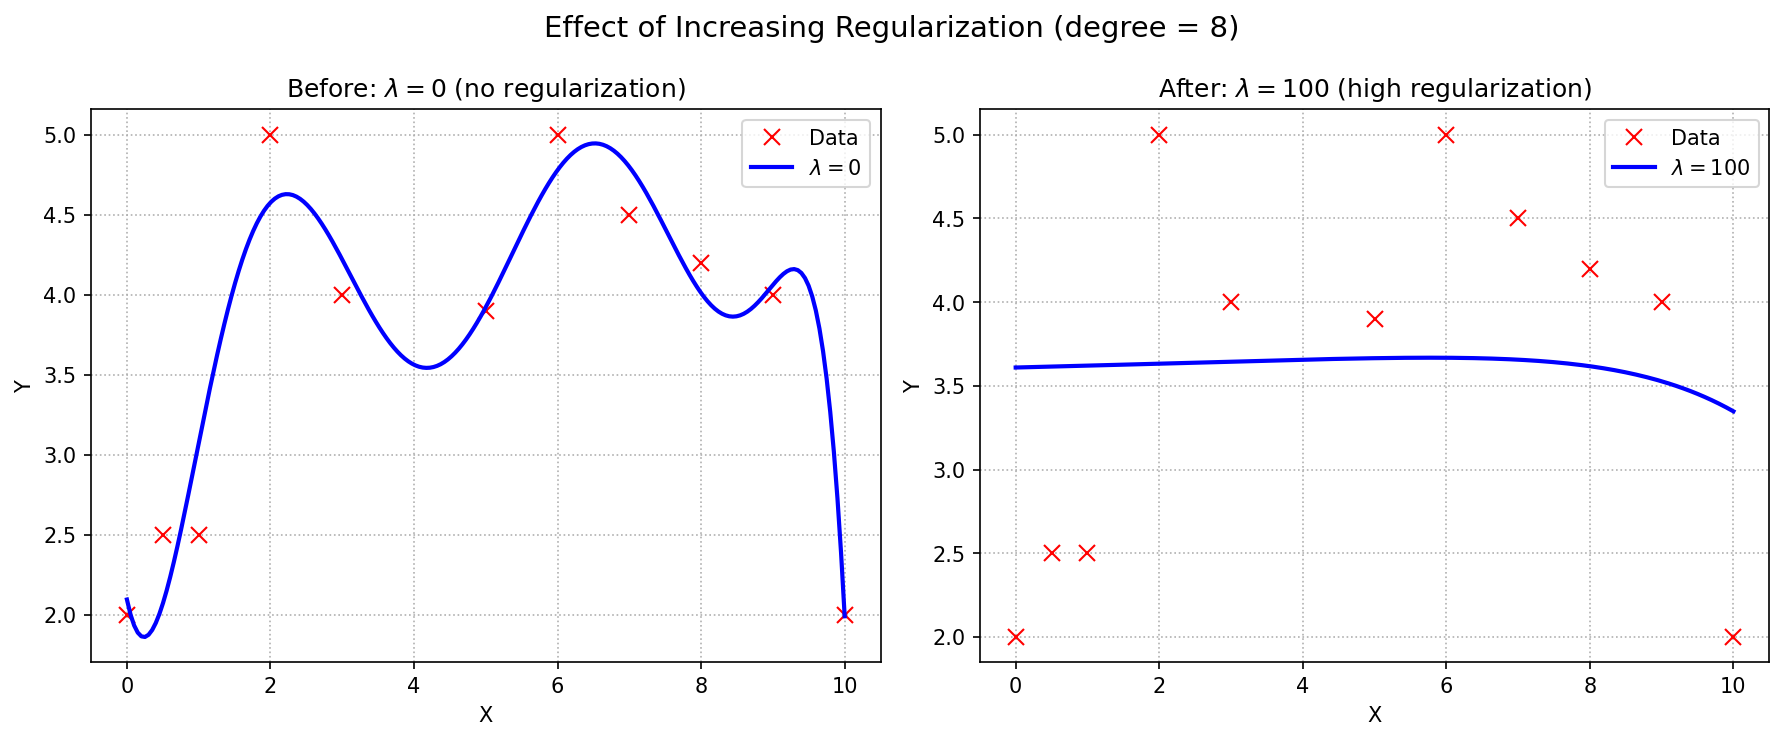
\includegraphics[width=\textwidth]{reg_effect.png}
    \caption{Degree-8 polynomial fit with $\lambda=0$ (left) versus $\lambda=100$ (right) on the polyreg dataset.}
\end{figure}

Increasing the regularization parameter $\lambda$ shrinks the model weights toward zero, causing the high-degree polynomial to produce a much smoother, flatter curve that trades variance for bias---eliminating the wild oscillations seen when $\lambda=0$ but at the cost of underfitting the underlying trend.

\section*{Learning Curves}

\begin{figure}[h]
    \centering
    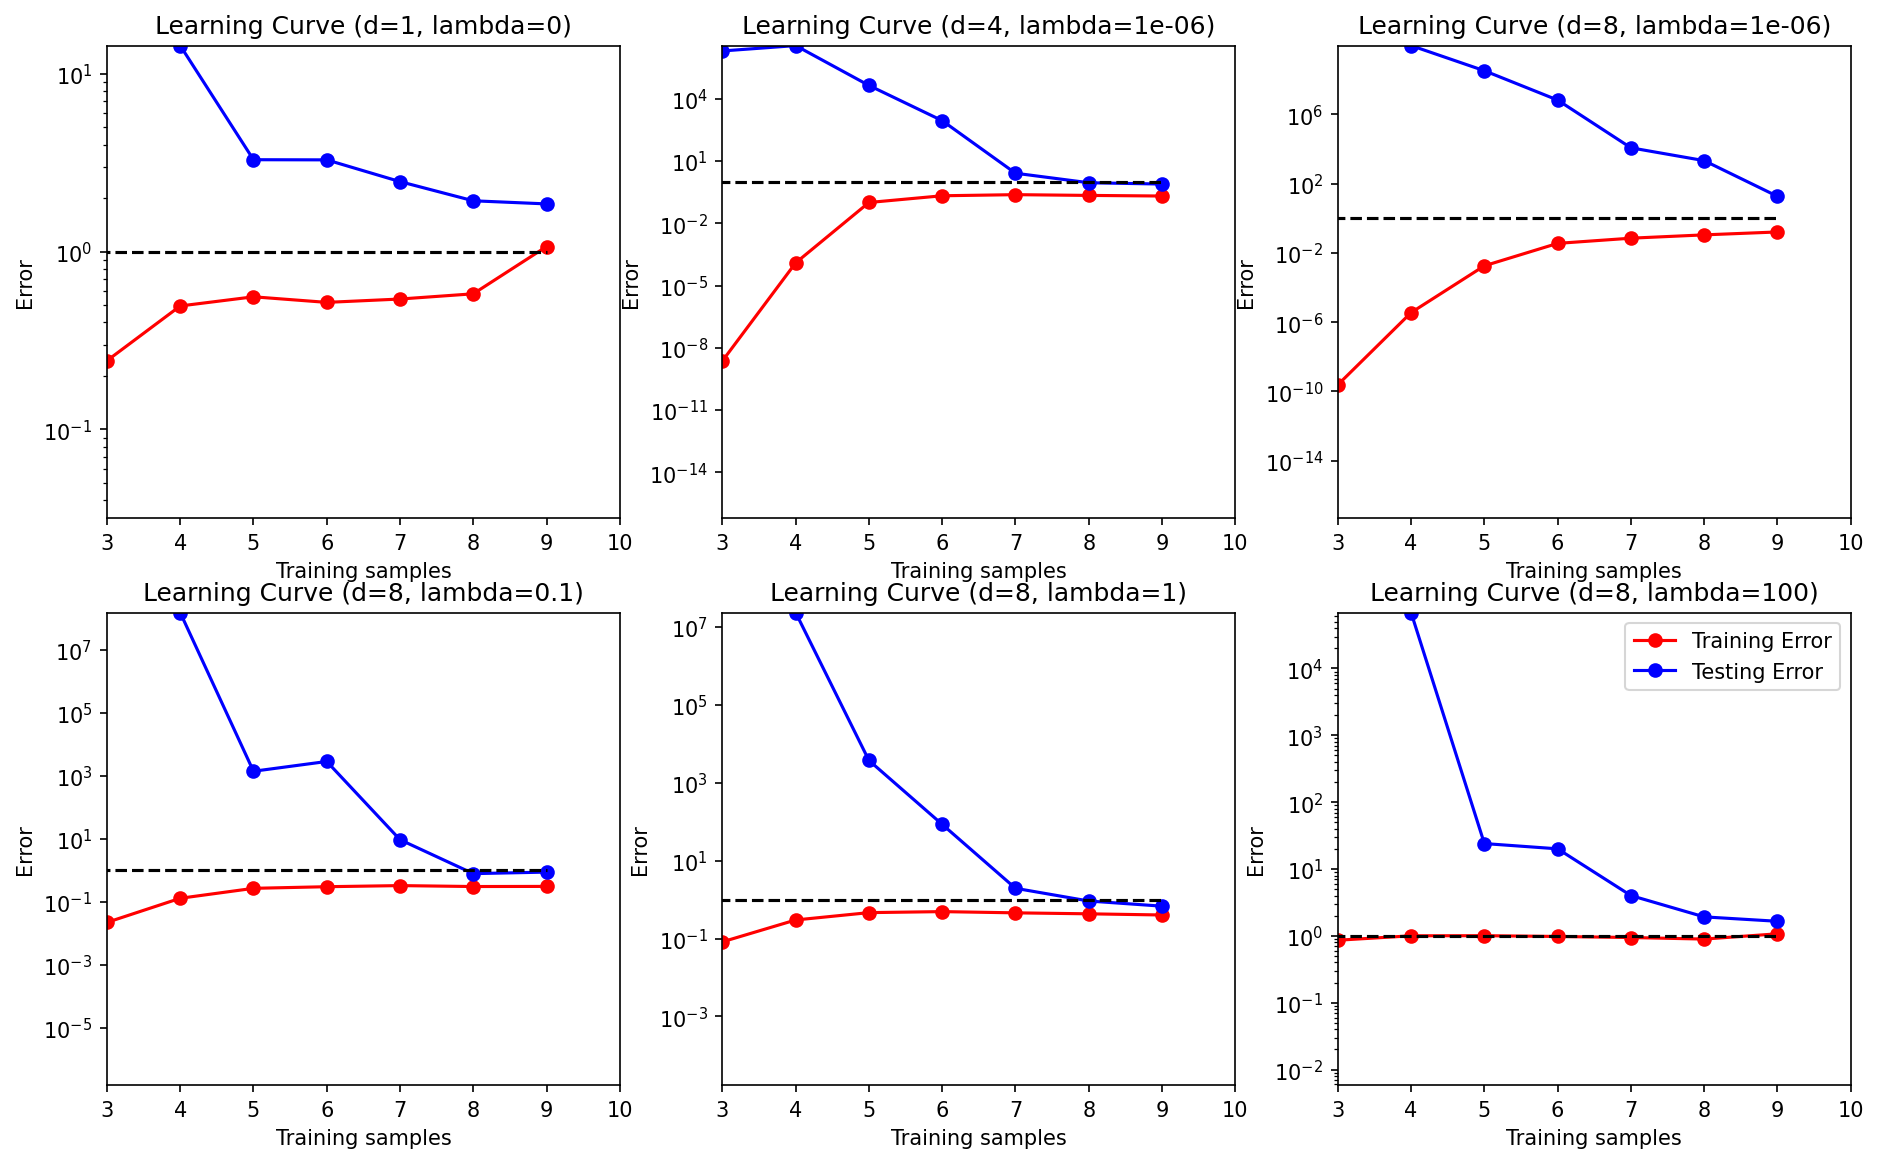
\includegraphics[width=\textwidth]{learning_curves.png}
    \caption{Learning curves (training error in red, test error in blue) for six combinations of polynomial degree $d$ and regularization $\lambda$.}
\end{figure}

As $\lambda$ increases from $10^{-6}$ to $100$ (degree $d=8$ panels), the gap between training and test error narrows because regularization reduces overfitting, but both errors converge to a higher floor, indicating that too much regularization introduces bias and prevents the model from capturing the true signal.

\end{document}
